\documentclass[12pt,english,twoside]{report}
\usepackage{mathptmx}
\renewcommand{\familydefault}{\rmdefault}
\usepackage[T1]{fontenc}
\usepackage[latin9]{inputenc}
\usepackage[a4paper]{geometry}
\setcounter{secnumdepth}{2} % Changed from 3 to 2. 0-chapter 1-section 2-subsection 
\setcounter{tocdepth}{2} % Changed from 3 to 2. 0-chapter 1-section 2-subsection 
\setlength{\parskip}{\medskipamount}
\setlength{\parindent}{0pt}
\usepackage{verbatim}
\usepackage{pdfpages}
\usepackage{graphicx}
\usepackage{subfig} %% This package has to be here

%Packages Added By George
\usepackage{setspace}
\usepackage{arabtex}
\usepackage[numbers]{natbib}
\usepackage{nomencl}
\usepackage{paralist}
\usepackage[linesnumbered]{algorithm2e}
\usepackage{color}
\usepackage{amsthm}
\usepackage[cmex10]{amsmath}
\usepackage{bbold}
\usepackage{multirow}
\usepackage{dsfont}
\usepackage{booktabs}
\usepackage{eufrak}
\usepackage{amssymb}

% Theorem Styles
\newtheorem{theorem}{Theorem}[section]
\newtheorem{lemma}[theorem]{Lemma}
\newtheorem{proposition}[theorem]{Proposition}
\newtheorem{corollary}[theorem]{Corollary}
% Definition Styles
\theoremstyle{definition}
\newtheorem{definition}{Definition}[section]
\newtheorem{example}{Example}[section]
\theoremstyle{remark}
\newtheorem{remark}{Remark}

\usepackage{etoolbox}
\newtoggle{edit-mode}
\togglefalse{edit-mode}  
%\toggletrue{edit-mode}

% the following is useful when we have the old nomencl.sty package
\providecommand{\printnomenclature}{\printglossary}
\providecommand{\makenomenclature}{\makeglossary}
\makenomenclature
\doublespacing

\makeatletter

%%%%%%%%%%%%%%%%%%%%%%%%%%%%%% User specified LaTeX commands.
\usepackage{tauthesis}
\iftoggle{edit-mode}{
\geometry{verbose,tmargin=2cm,bmargin=2cm,lmargin=2cm,rmargin=6cm,headheight=1cm,headsep=1cm,footskip=1cm, marginparwidth=5cm}
}

\usepackage[font={small,bf}, labelfont={small,bf}, margin=1cm]{caption}
\usepackage{titlesec}
\newcommand{\hsp}{\hspace{20pt}}
\titleformat{\chapter}[hang]{\Huge\bfseries}{\thechapter\hsp}{0pt}{\Huge\bfseries}

\University{Tel Aviv University}
\Faculty{The Iby and Aladar Fleischman Faculty of Engineering}
\School{The Zandman-Slaner School of Graduate Studies}
\Department {School of Mechanical Engineering}
\Title{\textbf{ \uppercase {Thesis Title}}}
\Degree{Master of Science in Engineering}
\Author{Your name}
\Year{September 2017}
\Supervisor{Prof. First Supervisor}
\SecondSupervisor{Dr. Second Supervisor}

\makeatother

\usepackage{babel}


\begin{document}


\pagenumbering{gobble}

\titlepage

\secondtitlepage

\dedication{\textbf{\emph{To my whomever, \\
for being whatever}}}

\acknowledgments{
\thispagestyle{empty}
This research would not have been possible without ...

A nice saying...


}

\cleardoublepage
\pagenumbering{roman}
\setcounter{page}{1} % Start preliminary pages numbering (roman numerals).


\chapter*{Abstract}
\vspace{-40pt}
Your abstract goes here....

\tableofcontents{}

\cleardoublepage

\addcontentsline{toc}{chapter}{Nomenclature}

\printnomenclature

\cleardoublepage

\listoffigures

\cleardoublepage

\listoftables

\textpages

%%%%%%%%%%% nomenclature %%%%%%%%%%
\nomenclature{TAU}{Tel aviv University}
\nomenclature{IIT}{Insrael institution of technology}
%%%%%%%%%%%%%%%%%%%%%%%%%%%%%%%%%%%%

\chapter{Introduction}

An example of a fully vocalised Arabic from the Qur'an (Al-Fatiha 1:1):
\begin{center}
\fullvocalize
\transtrue
\begin{RLtext}
bismi al-ll_ahi al-rra.hm_ani al-rra.hImi
\end{RLtext}
In the name of All'ah, the most gracious, the most merciful.
\end{center}

\iftoggle{edit-mode}{\hspace{0pt}\marginpar{Recognition-based segmentation}}{}




%%%%%%%%%%% Nomenclature for this chapter%%%%%%%%%%
\nomenclature{TAU}{Tel-Aviv University}



\chapter{Basic examples}
\label{chap:chapter 1}




%%%%%%%%%%%%%%%%%%%%%%%%%%%%%%%%%%%%
%%%%%%%%%%%%%%%%%%%%%%%%%%%%%%%%%%%%

\section{Examples}
\label{sec:examples}


Citations are very simple. Add all the references in the references files.
You can you Google scholar to easily copy the bibtex.
For instance, this paper \cite{kour2014real} is awsome.

See Figure \ref{fig:figure_label} as an example on how to add figures to your thesis.
It is recommended that all figures to be kept in a separate directory.
Note the `./figures/figure' in the example below.


\begin{figure}
\centering
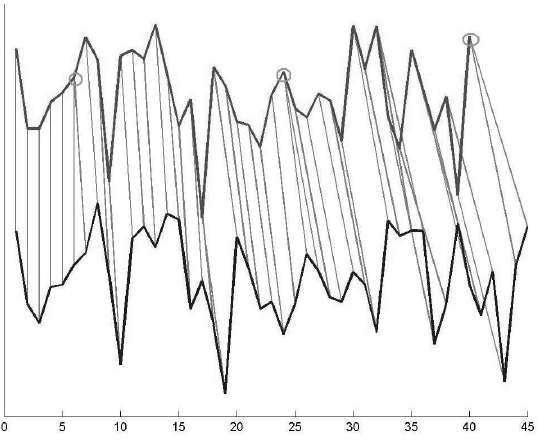
\includegraphics[width=0.5\textwidth]{./figures/figure}
\caption{A figure example.}
\label{fig:figure_label}
\end{figure}


See Table \ref{table:table_ex} to learn how to create tables.

\begin{table}
\centering
\caption{A table example}
\begin{tabular}{ c c c c }
\toprule
\textbf{Dataset} & \textbf{Number of samples} & \textbf{Results} & \textbf{Results 2} \\
\midrule                 
  Ini & 1405 & 48 & 9 \\ 
  Mid & 1196 & 52 & 10 \\ 
  Fin & 1629 & 44 & 9 \\ 
  Iso & 1372 & 39 & 8 \\ 
  \bottomrule
\end{tabular}
\label{table:table_ex} 
\end{table}

This how you create a new definition: go to \ref{def:distance_function}.

\begin{definition}
Given a data space $\mathfrak{D}$, for any two data elements $x,y \in \mathfrak{D}$, a \textbf{distance function} $dist$, on $\mathfrak{D}$ is defined as:
\begin{equation}
dist: \mathfrak{D} \times \mathfrak{D} \longrightarrow \mathds{R}_{\geq 0} 
\end{equation}
where $dist$ has the following properties:
\begin{compactitem}
\item $dist(x,y)=0 \Leftrightarrow x=y$ (reflexivity)
\item $dist(x,y) = dist(y,x)$ (symmetry)
\end{compactitem}
The pair $(\mathfrak{D},dist)$ is called a \textbf{distance space}.
\label{def:distance_function}
\end{definition}



\section {Nomenclature}

For updating nomenclature run the following commands:

makeindex Thesis-main.nlo -s nomencl.ist -o Thesis-main.nls

makeindex LettersClassification.nlo -s nomencl.ist -o LettersClassification.

\chapter{Summary, Conclusions and Future Work}

\begin{itemize}
\item item 1
\item item 2
\end{itemize}



\bibliographystyle{plainnat}
\bibliography{references}

\appendix

\chapter{Appendix 1}

appendix 1 content...

\cleardoublepage
\newpage
\thispagestyle{empty}
\mbox{}


\includepdf[pages=-]{hebrew_part}
\end{document}
